\chapter{Polygon Triangulation}
\label{ch:triangulations}

\section{Ear Clipping}
\label{sec:ear_clipping}

Ear clipping\index{ear clipping} is a simple and intuitive algorithm for triangulating a simple polygon. It is based on the Two-Ears Theorem, which states that every simple polygon with at least four vertices has at least two ``ears'' that can be removed to form a smaller simple polygon. By repeatedly clipping these ears, the entire polygon is eventually decomposed into triangles. The result was proved by Meisters~\cite{meisters1975}.

\subsection{Definitions}

\begin{definition}[Simple Polygon]\label{def:simple_polygon_tc}
A polygon is \emph{simple} if it does not self-intersect and has no holes.
\end{definition}

\begin{definition}[Convex Vertex]\label{def:convex_vertex}
A vertex $V_i$ of a polygon is \emph{convex} if the interior angle at $V_i$ is less than $\pi$ ($180^\circ$).
\end{definition}

\begin{definition}[Ear]\label{def:ear}
A vertex $V_i$ of a simple polygon is an \emph{ear}\index{ear} if the triangle formed by $V_{i-1}, V_i, V_{i+1}$ lies entirely within the polygon and contains no other vertices of the polygon in its interior.
\end{definition}

\begin{definition}[Barycentric Coordinates]\label{def:barycentric}
\emph{Barycentric coordinates}\index{barycentric coordinates} provide a coordinate system relative to a triangle. For a point $P$ and triangle $\triangle ABC$, the barycentric coordinates $(\lambda_1, \lambda_2, \lambda_3)$ satisfy $P = \lambda_1 A + \lambda_2 B + \lambda_3 C$ with $\lambda_1 + \lambda_2 + \lambda_3 = 1$ and $\lambda_i \ge 0$ if and only if $P$ lies inside $\triangle ABC$.
\end{definition}

\subsection{Theory}

The algorithm proceeds by identifying a vertex that satisfies two conditions:
\begin{enumerate}
\item The vertex is \textbf{convex} (the turn from $V_{i-1}$ to $V_i$ to $V_{i+1}$ is counter-clockwise for CCW polygons).
\item The triangle formed by $V_{i-1}, V_i, V_{i+1}$ contains no other vertices of the polygon in its interior.
\end{enumerate}

Once such an ear is found, the triangle $(V_{i-1}, V_i, V_{i+1})$ is recorded, and the vertex $V_i$ is removed from the polygon's vertex list. This process is repeated until only three vertices remain, which form the final triangle.

\begin{theorem}[Two-Ears Theorem]\label{thm:two_ears}
Every simple polygon with $n \ge 4$ vertices has at least two non-overlapping ears.
\end{theorem}

\begin{theorem}[Ear Clipping Correctness]\label{thm:ear_clipping_correctness}
The ear clipping algorithm produces a triangulation of any simple polygon with $n$ vertices, consisting of exactly $n - 2$ triangles.
\end{theorem}
\begin{proof}
We proceed by induction on $n$. For $n = 3$, the polygon is already a triangle. For $n \ge 4$, by the Two-Ears Theorem~\cite{meisters1975}, the polygon has at least one ear. Removing this ear produces a simple polygon with $n - 1$ vertices. By the inductive hypothesis, the smaller polygon can be triangulated into $(n-1) - 2 = n - 3$ triangles. Adding the ear triangle yields $n - 2$ triangles in total.
\end{proof}

\begin{figure}[htbp]
\centering
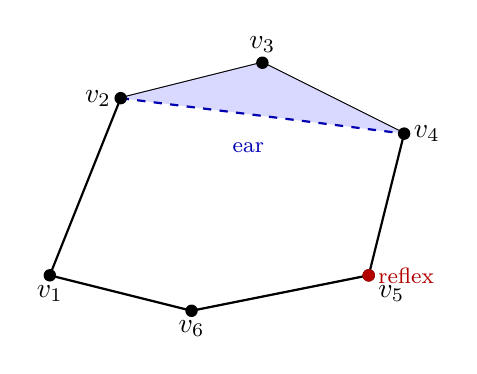
\begin{tikzpicture}[scale=0.9]
  \coordinate (A) at (0,0);
  \coordinate (B) at (1,2.5);
  \coordinate (C) at (3,3);
  \coordinate (D) at (5,2);
  \coordinate (E) at (4.5,0);
  \coordinate (F) at (2,-0.5);
  \draw[thick] (A)--(B)--(C)--(D)--(E)--(F)--cycle;
  \fill[blue!15] (B)--(C)--(D)--cycle;
  \draw[thick,blue!70!black,dashed] (B)--(D);
  \foreach \v/\name/\pos in {A/$v_1$/below,B/$v_2$/left,C/$v_3$/above,D/$v_4$/right,E/$v_5$/below right,F/$v_6$/below} {
    \fill (\v) circle (2.5pt) node[\pos] {\name};
  }
  \node[blue!70!black] at (2.8,1.8) {\footnotesize ear};
  \fill[red!70!black] (E) circle (2.5pt);
  \node[red!70!black,right] at (E) {\footnotesize reflex};
\end{tikzpicture}
\caption{Ear clipping: vertex $v_3$ is an ``ear'' since triangle $(v_2, v_3, v_4)$ is entirely inside the polygon and contains no other vertices.}
\label{fig:ear_clipping}
\end{figure}


\subsection{Pseudocode}

\begin{algorithm}[htbp]
\caption{Ear Clipping Triangulation}
\label{alg:ear_clipping}
\begin{algorithmic}[1]
\Function{Triangulate}{polygon}
  \State $indices \gets [0, 1, \ldots, n-1]$
  \State $triangles \gets [\,]$
  \While{$\text{len}(indices) > 3$}
    \For{$i = 0$ \textbf{to} $\text{len}(indices) - 1$}
      \State $u \gets indices[i-1]$
      \State $v \gets indices[i]$
      \State $w \gets indices[(i+1) \bmod \text{len}(indices)]$
      \If{$\text{IsEar}(u, v, w, indices, polygon)$}
        \State $triangles.\text{append}((u, v, w))$
        \State $indices.\text{pop}(i)$
        \State \textbf{break}
      \EndIf
    \EndFor
  \EndWhile
  \State $triangles.\text{append}(\text{tuple}(indices))$
  \State \Return $triangles$
\EndFunction

\Function{IsEar}{$u, v, w$, current\_indices, polygon}
  \If{$\text{cross\_product}(polygon[u], polygon[v], polygon[w]) \le 0$}
    \State \Return \textbf{False}
  \EndIf
  \For{index in current\_indices}
    \If{index $\in \{u, v, w\}$}
      \State \textbf{continue}
    \EndIf
    \If{$\text{PointInTriangle}(polygon[index], polygon[u], polygon[v], polygon[w])$}
      \State \Return \textbf{False}
    \EndIf
  \EndFor
  \State \Return \textbf{True}
\EndFunction
\end{algorithmic}
\end{algorithm}

\subsection{Parameters}

\begin{itemize}
\item \textbf{Input}: A list of \texttt{Point2D} representing a simple polygon in counter-clockwise order.
\item \textbf{Precision}: An epsilon should be used in cross-product and point-in-triangle tests to handle floating-point inaccuracies.
\end{itemize}

\subsection{Complexity}

\begin{itemize}
\item \textbf{Time Complexity}: $O(n^2)$\index{time complexity!$O(n^2)$} for a polygon with $n$ vertices. In each step, we check $O(n)$ vertices for ``ear-ness,'' and each check takes $O(n)$ time to verify that no other points are inside.
\item \textbf{Space Complexity}: $O(n)$ to store the triangles and the remaining vertex indices.
\end{itemize}

\begin{example}[Ear Clipping Trace]\label{ex:ear_clipping_trace}
Consider a quadrilateral with vertices (CCW): $V_0=(0,0)$, $V_1=(2,0)$, $V_2=(2,1)$, $V_3=(0,1)$. This is a convex rectangle, so every vertex is an ear.
\begin{enumerate}
\item Check $V_0$: $\operatorname{cross}(V_3, V_0, V_1) > 0$ and no other vertex is inside $\triangle V_3 V_0 V_1$. It is an ear.
\item Record triangle $(V_3, V_0, V_1)$ and remove $V_0$.
\item Remaining vertices: $V_1, V_2, V_3$ form a triangle.
\end{enumerate}
Result: Two triangles $(V_3, V_0, V_1)$ and $(V_1, V_2, V_3)$, which is the expected $n - 2 = 2$ triangles for a quadrilateral.
\end{example}

\subsection{Usages}

\begin{itemize}
\item Converting arbitrary polygons into triangles for rendering via OpenGL or DirectX.
\item Preprocessing geometry for physics simulation and collision detection.
\item Calculating the area or centroid of complex shapes.
\end{itemize}

\subsection{Testing and Edge Cases}

\begin{itemize}
\item \textbf{Concave Polygons}: Ensure the algorithm correctly skips reflex (non-convex) vertices.
\item \textbf{Collinear Vertices}: Handled by strict inequality in the convexity check.
\item \textbf{Self-intersecting Polygons}: Basic ear clipping may fail or produce incorrect results; the input must be simple.
\item \textbf{Sliver Triangles}: Very thin polygons can lead to numerical stability issues.
\item \textbf{Degenerate Polygons}: Polygons with 0, 1, or 2 vertices.
\end{itemize}

\subsection{References}

\begin{itemize}
\item Meisters, G. H. (1975). ``Polygons have ears''. The American Mathematical Monthly.
\item Eberly, D. (2002). ``Triangulation by Ear Clipping''. Geometric Tools.
\item Wikipedia: Polygon triangulation.
\end{itemize}


\section{Monotone Decomposition}
\label{sec:monotone_decomposition}

Monotone decomposition\index{monotone decomposition} is the process of partitioning a simple polygon into a set of monotone polygons. A polygon is monotone with respect to a line $L$ if every line orthogonal to $L$ intersects the polygon in at most one connected component (a single line segment). This is typically a preprocessing step for more efficient polygon triangulation, as monotone polygons can be triangulated in linear time~\cite{preparata1985}.

\subsection{Definitions}

\begin{definition}[Monotone Polygon]\label{def:monotone_polygon}
A polygon is \emph{monotone} with respect to a direction $d$ if every line orthogonal to $d$ intersects the polygon in at most one connected component (at most one line segment).
\end{definition}

\begin{definition}[Y-Monotone Polygon]\label{def:y_monotone}
A polygon is \emph{$y$-monotone} if every horizontal line intersects the interior in at most one connected component. Equivalently, the polygon has no ``cusp'' vertices where both neighbors have $y$-coordinates on the same side.
\end{definition}

\begin{definition}[Cusp Vertex]\label{def:cusp_vertex}
A \emph{cusp vertex}\index{cusp vertex} is a vertex where both adjacent vertices have $y$-coordinates either all above or all below it. Cusps violate $y$-monotonicity and are classified as:
\begin{itemize}
\item \textbf{Start/Split vertex}: interior is below, neighbors have higher $y$.
\item \textbf{End/Merge vertex}: interior is above, neighbors have lower $y$.
\end{itemize}
\end{definition}

\subsection{Theory}

The algorithm uses a \textbf{plane sweep}\index{plane sweep} approach, moving a horizontal line from top to bottom. The key to making a polygon $y$-monotone is to eliminate all split and merge vertices by adding diagonals. A split vertex is connected to a vertex above it (the ``helper'' of the edge to its left), and a merge vertex is connected to a vertex below it when the sweep line reaches it. By the time the sweep is finished, all cusps that violated monotonicity are resolved.

\begin{theorem}[Monotone Decomposition Correctness]\label{thm:monotone_decomp_correctness}
The sweep-line algorithm adds at most $r$ diagonals to produce a decomposition of a simple polygon with $r$ reflex vertices into at most $r + 1$ $y$-monotone sub-polygons.
\end{theorem}
\begin{proof}
Each split or merge vertex requires exactly one diagonal to resolve the cusp. There are at most $r$ such vertices (each reflex vertex is either a split, merge, or regular vertex; only split and merge vertices require diagonals). Adding one diagonal per such vertex resolves all monotonicity violations, yielding a partition into monotone pieces.
\end{proof}

\subsection{Pseudocode}

\begin{algorithm}[htbp]
\caption{Monotone Polygon Decomposition}
\label{alg:monotone_decomposition}
\begin{algorithmic}[1]
\Function{MonotoneDecomposition}{polygon}
  \State $events \gets \text{sorted}(polygon.vertices, \text{key}=\lambda v: (-v.y, v.x))$
  \State $status \gets \text{BalancedBST}()$
  \State $diagonals \gets [\,]$
  \For{$v$ in $events$}
    \If{$\text{IsStartVertex}(v)$}
      \State $\text{HandleStartVertex}(v, status)$
    \ElsIf{$\text{IsEndVertex}(v)$}
      \State $\text{HandleEndVertex}(v, status, diagonals)$
    \ElsIf{$\text{IsSplitVertex}(v)$}
      \State $\text{HandleSplitVertex}(v, status, diagonals)$
    \ElsIf{$\text{IsMergeVertex}(v)$}
      \State $\text{HandleMergeVertex}(v, status, diagonals)$
    \Else
      \State $\text{HandleRegularVertex}(v, status, diagonals)$
    \EndIf
  \EndFor
  \State \Return $\text{SplitPolygon}(polygon, diagonals)$
\EndFunction
\end{algorithmic}
\end{algorithm}

\subsection{Parameters}

\begin{itemize}
\item \textbf{Sweep Direction}: Usually vertical ($y$-axis), but can be any arbitrary direction if the polygon is rotated.
\item \textbf{Data Structures}: A balanced binary search tree (BST) for the status and a priority queue for events are standard.
\end{itemize}

\subsection{Complexity}

\begin{itemize}
\item \textbf{Time Complexity}: $O(n \log n)$ due to the sorting of vertices and the $O(\log n)$ operations on the balanced BST for each vertex.
\item \textbf{Space Complexity}: $O(n)$ to store the polygon, the status tree, and the resulting diagonals.
\end{itemize}

\subsection{Usages}

\begin{itemize}
\item \textbf{Triangulation}: The first stage of $O(n \log n)$ polygon triangulation algorithms.
\item \textbf{Trapezoidal Decomposition}: Often used in conjunction with monotone partitioning.
\item \textbf{Path Planning}: Simplifying complex obstacles into monotone regions for easier navigation.
\end{itemize}

\subsection{Testing and Edge Cases}

\begin{itemize}
\item \textbf{Horizontal Edges}: Vertices with identical $y$-coordinates require consistent tie-breaking in the sort.
\item \textbf{Complex Cusps}: Multiple split/merge vertices at the same height.
\item \textbf{Strict Monotonicity}: Ensuring that horizontal lines intersecting a vertex or edge are handled correctly.
\item \textbf{Non-Simple Polygons}: Monotone decomposition is generally defined for simple polygons; holes require special handling (treating them as merge/split events).
\end{itemize}

\subsection{References}

\begin{itemize}
\item Berg, M. de, Cheong, O., Kreveld, M. van, \& Overmars, M. (2008). ``Computational Geometry: Algorithms and Applications''. Springer-Verlag.
\item Lee, D. T., \& Preparata, F. P. (1977). ``Location of a point in a planar subdivision and its applications''. SIAM Journal on Computing.
\item Wikipedia: Monotone polygon.
\end{itemize}


\section{Incremental Delaunay Triangulation}
\label{sec:incremental_delaunay}

Incremental Delaunay triangulation\index{Delaunay triangulation} is a fundamental algorithm for constructing a Delaunay triangulation of a set of points in the plane. The algorithm builds the triangulation by adding points one at a time and locally updating the mesh to maintain the Delaunay property. It was independently proposed by Bowyer~\cite{bowyer1981} and Watson~\cite{watson1981}. It is valued for its relative simplicity and efficiency, especially when combined with spatial sorting techniques.

\subsection{Definitions}

\begin{definition}[Delaunay Property]\label{def:delaunay_property}
A triangulation of a point set $P$ is \emph{Delaunay}\index{Delaunay property} if the circumcircle of every triangle contains no other point of $P$ in its interior.
\end{definition}

\begin{definition}[In-Circle Test]\label{def:incircle_test}
The \emph{in-circle test}\index{in-circle test} determines whether a point $D$ lies inside, on, or outside the circumcircle of triangle $ABC$. Given the determinant:
\[
\operatorname{InCircle}(A,B,C,D) = \begin{vmatrix}
a_x - d_x & a_y - d_y & (a_x - d_x)^2 + (a_y - d_y)^2 \\
b_x - d_x & b_y - d_y & (b_x - d_x)^2 + (b_y - d_y)^2 \\
c_x - d_x & c_y - d_y & (c_x - d_x)^2 + (c_y - d_y)^2
\end{vmatrix}
\]
the sign indicates: positive (inside), zero (on), negative (outside), assuming counter-clockwise orientation of $ABC$.
\end{definition}

\begin{definition}[Edge Flip]\label{def:edge_flip}
An \emph{edge flip}\index{edge flip} replaces the common edge of two adjacent triangles in a triangulation with the other diagonal of their union quadrilateral.
\end{definition}

\subsection{Theory}

The algorithm relies on the fact that any triangulation can be converted into a Delaunay triangulation through a series of edge flips. When a new point $P$ is inserted into a triangle $T$, it is connected to the three vertices of $T$, creating three new triangles. The edges of these new triangles (which were the edges of $T$) may now be ``illegal.'' The algorithm recursively checks and flips these edges until the Delaunay property is restored globally.

\begin{theorem}[Delaunay Triangulation Existence and Uniqueness]\label{thm:delaunay_existence}
For a set of $n$ points in $\mathbb{R}^2$ in general position (no four points co-circular), the Delaunay triangulation exists and is unique.
\end{theorem}

\begin{theorem}[Incremental Delaunay Correctness]\label{thm:incremental_delaunay_correctness}
The incremental insertion algorithm with edge legalization produces a valid Delaunay triangulation.
\end{theorem}
\begin{proof}
The proof proceeds by induction on the number of inserted points. After inserting the first three points, the single triangle trivially satisfies the Delaunay property. When point $p$ is inserted into triangle $T$, the three new triangles may violate the Delaunay property only along the edges shared with neighboring triangles. The \textsc{LegalizeEdge} procedure checks the in-circle condition for each such edge. If violated, flipping the edge locally restores the Delaunay property for that edge. Since each flip can only create at most two new potentially illegal edges (among the new neighbors), the process terminates. The total number of flips is $O(n)$ in the expected case.
\end{proof}

\subsection{Pseudocode}

\begin{algorithm}[htbp]
\caption{Incremental Delaunay Triangulation}
\label{alg:incremental_delaunay}
\begin{algorithmic}[1]
\Function{IncrementalDelaunay}{points}
  \State $ST \gets \text{CreateSuperTriangle}(points)$
  \State $Triangulation \gets \{ST\}$
  \For{$p$ in $points$}
    \State $T \gets \text{FindTriangleContaining}(p, Triangulation)$
    \State $\text{SplitTriangle}(T, p, Triangulation)$
  \EndFor
  \State $\text{RemoveSuperTriangleVertices}(Triangulation)$
  \State \Return $Triangulation$
\EndFunction

\Function{SplitTriangle}{$T$, $p$, Triangulation}
  \State $(A, B, C) \gets T.vertices$
  \State $NewTris \gets [(p, A, B), (p, B, C), (p, C, A)]$
  \State Replace $T$ with $NewTris$ in $Triangulation$
  \For{each $edge$ in $\{AB, BC, CA\}$}
    \State $\text{LegalizeEdge}(p, edge, Triangulation)$
  \EndFor
\EndFunction

\Function{LegalizeEdge}{$p$, $edge(U, V)$, Triangulation}
  \State $Neighbor \gets \text{FindNeighbor}(edge, Triangulation)$
  \If{$Neighbor$ is None}
    \State \Return
  \EndIf
  \State $W \gets Neighbor.\text{vertex\_opposite\_to}(edge)$
  \If{$\text{InCircle}(p, U, V, W)$}
    \State $\text{FlipEdge}(edge(U, V))$ to $edge(p, W)$
    \State $\text{LegalizeEdge}(p, edge(U, W), Triangulation)$
    \State $\text{LegalizeEdge}(p, edge(W, V), Triangulation)$
  \EndIf
\EndFunction
\end{algorithmic}
\end{algorithm}

\subsection{Parameters}

\begin{itemize}
\item \textbf{Point Location}: Using a \textbf{Visibility Walk} or a \textbf{Point Grid} (spatial index) drastically speeds up finding the triangle containing the new point.
\item \textbf{Insertion Order}: Sorting points along a \textbf{Hilbert Curve} or \textbf{Morton Code} ensures that subsequent points are geographically close, keeping the walk short.
\end{itemize}

\subsection{Complexity}

\begin{itemize}
\item \textbf{Time Complexity}: Average case $O(n \log n)$\index{time complexity!$O(n \log n)$} with spatial sorting and efficient point location. Worst case $O(n^2)$\index{time complexity!$O(n^2)$} for highly structured point sets without randomization or sorting.
\item \textbf{Space Complexity}: $O(n)$ to store the triangles and point coordinates.
\end{itemize}

\subsection{Usages}

\begin{itemize}
\item Generating high-quality meshes for Finite Element Method (FEM) analysis.
\item Interpolation of scattered data (e.g., creating contour maps from elevation points).
\item Pathfinding in robotics and video games.
\item Dual representation of Voronoi diagrams\index{Voronoi diagram}.
\end{itemize}

\subsection{Testing and Edge Cases}

\begin{itemize}
\item \textbf{Co-circular Points}: Four or more points on the same circle. The algorithm will choose one valid triangulation, but the result may not be unique.
\item \textbf{Collinear Points}: Points lying on a single line. Requires robust predicates or a small perturbation (epsilon).
\item \textbf{Points on Edges}: If a point falls exactly on an existing edge, the edge should be split into four triangles instead of three.
\item \textbf{Super-Triangle Selection}: Must be large enough to contain all points, but not so large that it causes numerical overflow.
\end{itemize}

\subsection{References}

\begin{itemize}
\item Bowyer, A. (1981). ``Computing Dirichlet tessellations''. The Computer Journal.
\item Watson, D. F. (1981). ``Computing the n-dimensional Delaunay tessellation with application to Voronoi polytopes''. The Computer Journal.
\item Guibas, L., \& Stolfi, J. (1985). ``Primitives for the manipulation of general subdivisions and the computation of Voronoi diagrams''. ACM Transactions on Graphics.
\item Wikipedia: Delaunay triangulation.
\end{itemize}


\section{Dynamic Delaunay Triangulation}
\label{sec:dynamic_delaunay}

Dynamic Delaunay triangulation is the process of maintaining a Delaunay triangulation as points are inserted into or deleted from the set. Unlike static construction, where the entire point set is known beforehand, dynamic algorithms must update the mesh locally to restore the Delaunay property while maintaining efficiency. This is critical for applications involving moving objects, real-time data streams, and interactive geometry editing.

\subsection{Definitions}

\begin{definition}[Dynamic Triangulation]\label{def:dynamic_triangulation}
A \emph{dynamic triangulation} maintains a valid triangulation under a sequence of point insertions and deletions, guaranteeing the triangulation invariant (here, the Delaunay property) after each update.
\end{definition}

\subsection{Theory}

\subsubsection*{Insertion}

Insertion typically uses the \textbf{Incremental Algorithm} (\cref{alg:incremental_delaunay}):
\begin{enumerate}
\item \textbf{Locate}: Find triangle $T$ containing new point $P$.
\item \textbf{Split}: Split $T$ into three new triangles by connecting $P$ to its vertices.
\item \textbf{Legalize}: Recursively check the edges of the new triangles and perform \textbf{Delaunay Flips} until all edges are legal (satisfy the empty circumcircle property).
\end{enumerate}

\subsubsection*{Deletion}

Deletion is more complex:
\begin{enumerate}
\item \textbf{Remove}: Remove the vertex $V$ and all incident edges, leaving a star-shaped polygon (the ``hole'').
\item \textbf{Re-triangulate}: Triangulate the hole. A simple way is to use a recursive ``ear clipping'' approach that specifically chooses diagonals satisfying the Delaunay property.
\item \textbf{Legalize}: Alternatively, perform any triangulation of the hole and then flip edges until it is Delaunay.
\end{enumerate}

\begin{theorem}[Expected Flip Complexity]\label{thm:expected_flips}
For $n$ points inserted in random order, the total number of edge flips during incremental Delaunay triangulation is $O(n)$ in expectation.
\end{theorem}
\begin{proof}
Guibas, Knuth, and Sharir~\cite{guibas1985} showed that the randomized analysis of edge flips leads to an amortized $O(1)$ flips per insertion. The key observation is that each flip can be ``charged'' to a pair of points whose circumcircle relation changes, and the total number of such chargeable events is bounded by $O(n)$ by a planar graph argument.
\end{proof}

\subsection{Pseudocode}

\subsubsection*{Dynamic Insertion}

\begin{algorithm}[htbp]
\caption{Dynamic Point Insertion}
\label{alg:dynamic_insertion}
\begin{algorithmic}[1]
\Function{InsertPoint}{triangulation, $p$}
  \State $T \gets \text{FindTriangleContaining}(triangulation, p)$
  \State $new\_triangles \gets \text{SplitTriangle}(T, p)$
  \State $edges\_to\_check \gets \text{GetOuterEdges}(new\_triangles)$
  \While{$edges\_to\_check$ is not empty}
    \State $e \gets edges\_to\_check.\text{pop}()$
    \If{$\text{IsIllegal}(e, triangulation)$}
      \State $new\_e \gets \text{Flip}(e, triangulation)$
      \State $edges\_to\_check.\text{extend}(\text{GetSurroundingEdges}(new\_e))$
    \EndIf
  \EndWhile
\EndFunction
\end{algorithmic}
\end{algorithm}

\subsubsection*{Dynamic Deletion}

\begin{algorithm}[htbp]
\caption{Dynamic Point Deletion}
\label{alg:dynamic_deletion}
\begin{algorithmic}[1]
\Function{DeletePoint}{triangulation, $v$}
  \State $neighbors \gets \text{GetAdjacentVertices}(v, triangulation)$
  \State $\text{RemoveVertex}(v, triangulation)$
  \State $\text{FillHoleDelaunay}(neighbors, triangulation)$
\EndFunction
\end{algorithmic}
\end{algorithm}

\subsection{Parameters}

\begin{itemize}
\item \textbf{Point Location Strategy}: For high performance, use a \textbf{Stochastic Walk} or a \textbf{Directed Acyclic Graph (DAG)} (e.g., the Delaunay Tree) to achieve $O(\log n)$ location time.
\item \textbf{Robustness}: Use robust predicates to prevent infinite loops during flipping caused by precision errors.
\end{itemize}

\subsection{Complexity}

\begin{itemize}
\item \textbf{Insertion}: $O(\log n)$ average for location, $O(1)$ expected for flipping (though $O(n)$ worst-case).
\item \textbf{Deletion}: $O(\log n)$ average to find the vertex, $O(k)$ to re-triangulate where $k$ is the degree of the vertex.
\item \textbf{Space}: $O(n)$ to store the triangles and point location structures.
\end{itemize}

\subsection{Usages}

\begin{itemize}
\item \textbf{Terrain Modeling}: Adding new survey points to a digital elevation model.
\item \textbf{Robotics}: Updating a map as a robot moves and discovers new obstacles.
\item \textbf{Fluid Simulation}: Re-meshing around a moving boundary (e.g., a boat moving through water).
\item \textbf{Mesh Refinement}: Splitting triangles to improve resolution in high-gradient areas.
\item \textbf{Data Visualization}: Real-time plotting of scattered data points.
\end{itemize}

\subsection{Testing and Edge Cases}

\begin{itemize}
\item \textbf{Co-circular Points}: Ensure both insertion and deletion handle cases where four or more points lie on a circle (Delaunay triangulation is not unique).
\item \textbf{Points on Boundary}: Handle points added to or removed from the convex hull correctly.
\item \textbf{Degenerate Deletion}: Deleting a vertex that reduces the convex hull to a line or a single point.
\item \textbf{Multiple Insertions at same position}: Handle duplicate points by ignoring them or updating metadata.
\item \textbf{High-Valence Vertices}: Test deletion of vertices shared by many (e.g., 50+) triangles.
\end{itemize}

\subsection{References}

\begin{itemize}
\item Bowyer, A. (1981). ``Computing Dirichlet tessellations''. The Computer Journal.
\item Watson, D. F. (1981). ``Computing the n-dimensional Delaunay tessellation with application to Voronoi polytopes''. The Computer Journal.
\item Guibas, L., Knuth, D. E., \& Sharir, M. (1992). ``Randomized incremental construction of Delaunay and Voronoi diagrams''. Algorithmica.
\item Devillers, O. (1999). ``On handling transitions between different structures in geometric modeling''. Proceedings of the 11th Canadian Conference on Computational Geometry.
\item Wikipedia: Delaunay triangulation.
\end{itemize}


\section{Delaunay Flips}
\label{sec:delaunay_flips}

The edge flip algorithm is a local transformation technique used to convert any valid triangulation of a set of points into a \textbf{Delaunay triangulation}. It is based on the Lawson Flip Theorem~\cite{lawson1977}, which states that any two triangulations of the same set of points are connected by a series of edge flips. This process iteratively improves the ``quality'' of the triangles by ensuring they satisfy the Delaunay (empty circumcircle) property.

\subsection{Definitions}

\begin{definition}[Illegal Edge]\label{def:illegal_edge}
An interior edge $e$ shared by triangles $T_1 = (A, B, C)$ and $T_2 = (B, C, D)$ is \emph{illegal}\index{illegal edge} if $D$ lies inside the circumcircle of $\triangle ABC$ (equivalently, if $\operatorname{InCircle}(A, B, C, D) > 0$).
\end{definition}

\begin{definition}[Angle-Vector]\label{def:angle_vector}
The \emph{angle-vector} of a triangulation is the sorted (non-decreasing) list of all interior angles. Delaunay flips lexicographically maximize this vector, yielding the triangulation that maximizes the minimum angle.
\end{definition}

\subsection{Theory}

For any interior edge $e$ shared by triangles $T_1 = (A, B, C)$ and $T_2 = (B, C, D)$, we check the \textbf{In-Circle} condition for vertex $D$ relative to triangle $ABC$. If $D$ is inside the circumcircle of $ABC$, then the edge $BC$ is illegal.

Flipping an illegal edge $BC$ produces a new edge $AD$ and two new triangles $ABD$ and $ACD$. It is a proven property that:
\begin{enumerate}
\item Flipping an illegal edge increases the minimum angle of the triangulation.
\item An illegal edge can only exist if the four vertices form a convex quadrilateral.
\item By repeatedly flipping illegal edges, the algorithm will eventually converge to the unique Delaunay triangulation (assuming no four points are co-circular).
\end{enumerate}

\begin{theorem}[Lawson's Flip Theorem]\label{thm:lawson_flip}
Any triangulation of a point set in general position can be transformed into the Delaunay triangulation by a finite sequence of edge flips. Furthermore, the number of flips is at most $O(n^2)$.
\end{theorem}
\begin{proof}
Each flip strictly increases the angle-vector in lexicographic order. Since there are finitely many triangulations of $n$ points (at most $O(27^n)$ by a result of Sharir and others), the process must terminate. The bound of $O(n^2)$ flips follows from an amortized analysis of the number of illegal edges created per flip.
\end{proof}

\begin{figure}[htbp]
\centering
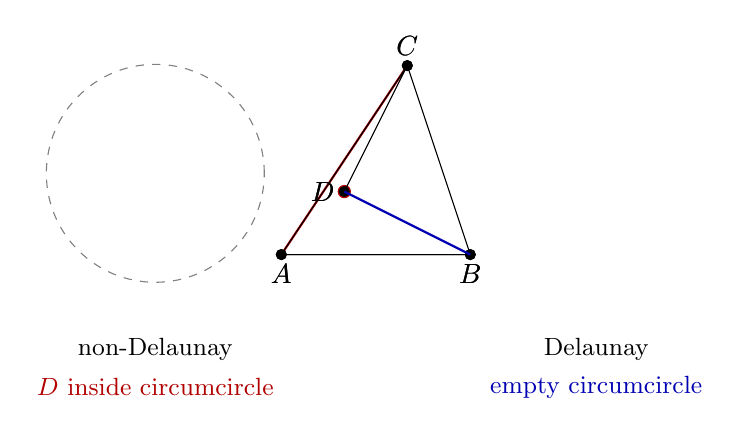
\begin{tikzpicture}[scale=0.8]
  \coordinate (A) at (0,0);
  \coordinate (B) at (3,0);
  \coordinate (C) at (2,3);
  \coordinate (D) at (1,1);
  \begin{scope}[xshift=-3.5cm]
    \fill (A) circle (2.5pt) node[below] {$A$};
    \fill (B) circle (2.5pt) node[below] {$B$};
    \fill (C) circle (2.5pt) node[above] {$C$};
    \fill (D) circle (2.5pt) node[left] {$D$};
    \draw (A)--(B)--(C)--cycle;
    \draw[red!70!black,thick] (A)--(C);
    \draw[gray,dashed] (1.5,1.29) circle (1.73);
    \fill[red!70!black] (D) circle (3pt);
    \node at (1.5,-1.5) {\small non-Delaunay};
    \node[red!70!black] at (1.5,-2.1) {\small $D$ inside circumcircle};
  \end{scope}
  \begin{scope}[xshift=3.5cm]
    \fill (A) circle (2.5pt) node[below] {$A$};
    \fill (B) circle (2.5pt) node[below] {$B$};
    \fill (C) circle (2.5pt) node[above] {$C$};
    \fill (D) circle (2.5pt) node[left] {$D$};
    \draw (A)--(B)--(D)--(C)--cycle;
    \draw[blue!70!black,thick] (B)--(D);
    \node at (1.5,-1.5) {\small Delaunay};
    \node[blue!70!black] at (1.5,-2.1) {\small empty circumcircle};
  \end{scope}
\end{tikzpicture}
\caption{Delaunay property: (left)~edge $AC$ is illegal because $D$ lies inside the circumcircle of $ABC$. (right)~Flipping to edge $BD$ satisfies the empty circumcircle property.}
\label{fig:delaunay_flip}
\end{figure}


\subsection{Pseudocode}

\begin{algorithm}[htbp]
\caption{Delaunay Edge Flip Algorithm}
\label{alg:delaunay_flip}
\begin{algorithmic}[1]
\Function{DelaunayFlip}{triangulation}
  \State $illegal\_edges \gets \text{Queue}()$
  \For{$edge$ in triangulation.interior\_edges}
    \If{$\text{IsIllegal}(edge, triangulation)$}
      \State $illegal\_edges.\text{push}(edge)$
    \EndIf
  \EndFor
  \While{$illegal\_edges$ is not empty}
    \State $edge \gets illegal\_edges.\text{pop}()$
    \If{$\text{IsIllegal}(edge, triangulation)$}
      \State $new\_edge \gets \text{Flip}(edge, triangulation)$
      \For{$neighbor$ in $\text{GetNeighboringEdges}(new\_edge)$}
        \If{$neighbor.\text{is\_interior}$}
          \State $illegal\_edges.\text{push}(neighbor)$
        \EndIf
      \EndFor
    \EndIf
  \EndWhile
  \State \Return $triangulation$
\EndFunction

\Function{IsIllegal}{$edge(B,C)$, triangulation}
  \State $T1 \gets triangulation.\text{GetFace}(edge)$
  \State $T2 \gets triangulation.\text{GetOppositeFace}(edge)$
  \State $A \gets T1.\text{vertex\_opposite}(edge)$
  \State $D \gets T2.\text{vertex\_opposite}(edge)$
  \State \Return $\text{InCircle}(A, B, C, D)$
\EndFunction
\end{algorithmic}
\end{algorithm}

\subsection{Parameters}

\begin{itemize}
\item \textbf{Robust Predicates}: The \texttt{InCircle} test must be implemented using robust geometric predicates (e.g., using \texttt{orient2d} and \texttt{incircle} from Shewchuk~\cite{shewchuk1997}) to handle floating-point precision issues.
\item \textbf{Data Structure}: A \textbf{Half-Edge} or \textbf{Quad-Edge}\index{quad-edge data structure} data structure is essential for efficiently finding neighboring faces and edges.
\end{itemize}

\subsection{Complexity}

\begin{itemize}
\item \textbf{Time Complexity}: In the worst case, $O(n^2)$\index{time complexity!$O(n^2)$} flips may be required for $n$ points. However, starting from a ``good'' initial triangulation (like one from a sweep-line), it is often much faster.
\item \textbf{Space Complexity}: $O(n)$ to store the triangulation and the queue of edges.
\end{itemize}

\subsection{Usages}

\begin{itemize}
\item \textbf{Mesh Refinement}: Improving the quality of an existing mesh for Finite Element analysis.
\item \textbf{Incremental Construction}: Maintaining a Delaunay triangulation as points are added or moved.
\item \textbf{Terrain Modeling}: Converting a set of elevation samples into a high-quality TIN (Triangulated Irregular Network).
\item \textbf{Fluid Simulation}: Re-meshing to avoid thin, sliver triangles that cause numerical instability.
\end{itemize}

\subsection{Testing and Edge Cases}

\begin{itemize}
\item \textbf{Co-circular Points}: Four points on a circle mean both diagonals are ``legal.'' The algorithm should terminate consistently.
\item \textbf{Non-Convex Quadrilateral}: Ensure the flip logic only applies to convex quadrilaterals (though an illegal edge is guaranteed to be a diagonal of a convex quad).
\item \textbf{Boundary Edges}: Edges on the convex hull cannot be flipped.
\item \textbf{Sliver Triangles}: Verify that flips successfully remove extremely thin triangles.
\item \textbf{Convergence}: Test on highly structured point sets (like a grid) to ensure the algorithm doesn't loop infinitely due to precision errors.
\end{itemize}

\subsection{References}

\begin{itemize}
\item Lawson, C. L. (1977). ``Software for $C^1$ surface interpolation''. Mathematical Software.
\item Guibas, L., \& Stolfi, J. (1985). ``Primitives for the manipulation of general subdivisions and the computation of Voronoi diagrams''. ACM Transactions on Graphics.
\item Shewchuk, J. R. (1997). ``Adaptive Precision Floating-Point Arithmetic and Fast Robust Geometric Predicates''. Discrete \& Computational Geometry.
\item Wikipedia: Delaunay triangulation.
\end{itemize}


\section{Constrained Delaunay Triangulation}
\label{sec:constrained_delaunay}

Constrained Delaunay Triangulation (CDT)\index{constrained Delaunay triangulation} is a version of Delaunay triangulation that forces certain edges (constraints) into the triangulation. It is essential for representing domains with specific boundaries, holes, or internal features that must be preserved.

\subsection{Overview}

While a standard Delaunay triangulation maximizes the minimum angle and satisfies the ``empty circumcircle'' property for all points, it may not respect the boundaries of a non-convex polygon. CDT modifies the Delaunay criteria to ensure that all constraint edges are present in the final mesh, while maintaining the Delaunay property for all other edges as much as possible.

\subsection{Implementation Details}

The CDT is implemented using an iterative edge-flip approach:
\begin{enumerate}
\item \textbf{Initial Triangulation}: The domain (including holes) is initially triangulated using a standard polygon triangulation algorithm.
\item \textbf{Constraint Enforcement}: Bridge edges are added to connect holes to the outer boundary, creating a single degenerate polygon that is then triangulated.
\item \textbf{Edge Flipping}: All internal edges that are not part of the constraints are placed in a queue. Edges are flipped if they violate the Delaunay condition, provided the flip doesn't cross a constraint and maintains the domain's validity.
\end{enumerate}

\subsection{Pseudocode}

\begin{algorithm}[htbp]
\caption{Constrained Delaunay Triangulation}
\label{alg:cdt}
\begin{algorithmic}[1]
\Function{ConstrainedDelaunayTriangulation}{outer, holes}
  \State $triangulation \gets \text{TriangulateDomain}(outer, holes)$
  \State $edge\_queue \gets \text{GetInteriorNonConstraintEdges}(triangulation)$
  \While{$edge\_queue$ is not empty}
    \State $e \gets edge\_queue.\text{pop}()$
    \If{$\text{IsIllegal}(e)$ \textbf{and} $\neg\, \text{CrossesConstraint}(e)$}
      \State $\text{Flip}(e, triangulation)$
      \State $edge\_queue.\text{extend}(\text{GetAffectedEdges}(e))$
    \EndIf
  \EndWhile
  \State \Return $triangulation$
\EndFunction
\end{algorithmic}
\end{algorithm}

\subsection{Usage Example}

\begin{verbatim}
from compgeom.mesh import constrained_delaunay_triangulation
from compgeom import Point2D

outer = [Point2D(0,0), Point2D(10,0), Point2D(10,10), Point2D(0,10)]
holes = [[Point2D(4,4), Point2D(6,4), Point2D(6,6), Point2D(4,6)]]

triangles, constrained_edges = constrained_delaunay_triangulation(outer, holes)
\end{verbatim}

\subsection{References}

\begin{itemize}
\item Chew, L. Paul. ``Constrained Delaunay Triangulations.'' Algorithmica, 1989.
\item Sloan, S. W. ``A Fast Algorithm for Generating Constrained Delaunay Triangulations.'' Computers \& Structures, 1993.
\end{itemize}


\section{Non-Obtuse Triangulation}
\label{sec:non_obtuse_triangulation}

Non-Obtuse Triangulation\index{non-obtuse triangulation} is the process of subdividing a 2D domain into triangles such that no internal angle exceeds $90^\circ$.

\subsection{Overview}

Most standard triangulation algorithms (including Delaunay) may produce obtuse triangles. For certain numerical simulations (like finite element analysis or fluid dynamics), obtuse triangles can introduce errors or numerical instability. A non-obtuse triangulation ensures that all angles are acute or right angles.

\subsection{Implementation Details}

The \texttt{NonObtuseTriangulator} uses an iterative Steiner point\index{Steiner point} insertion strategy:
\begin{enumerate}
\item \textbf{Initial Mesh}: Start with a Delaunay triangulation of the input point set.
\item \textbf{Detection}: Identify triangles with an angle $> 90^\circ$.
\item \textbf{Refinement}: For each obtuse triangle, insert a new vertex (Steiner point) at the midpoint of its longest edge.
\item \textbf{Re-triangulation}: Update the Delaunay triangulation with the new point.
\item \textbf{Iteration}: Repeat until no obtuse triangles remain or a maximum number of Steiner points is reached.
\end{enumerate}

\subsection{Pseudocode}

\begin{algorithm}[htbp]
\caption{Non-Obtuse Triangulation}
\label{alg:non_obtuse}
\begin{algorithmic}[1]
\Function{NonObtuseTriangulate}{points, max\_steiner}
  \State $mesh \gets \text{DelaunayTriangulation}(points)$
  \State $steiner\_count \gets 0$
  \While{$\text{hasObtuse}(mesh)$ \textbf{and} $steiner\_count < max\_steiner$}
    \State $T \gets \text{findObtuseTriangle}(mesh)$
    \State $edge \gets \text{longestEdge}(T)$
    \State $midpoint \gets \text{midpoint}(edge)$
    \State $\text{InsertPoint}(mesh, midpoint)$
    \State $steiner\_count \gets steiner\_count + 1$
  \EndWhile
  \State \Return $mesh$
\EndFunction
\end{algorithmic}
\end{algorithm}

\subsection{Usage Example}

\begin{verbatim}
from compgeom.mesh.surface.trimesh.non_obtuse_triangulation import NonObtuseTriangulator
from compgeom import Point2D

pts = [Point2D(0, 0), Point2D(10, 0), Point2D(5, 0.1)]
triangulator = NonObtuseTriangulator(pts)
mesh = triangulator.triangulate(max_steiner=100)
\end{verbatim}

\subsection{References}

\begin{itemize}
\item Bern, M., et al. ``Provably Good Mesh Generation.'' Journal of Computer and System Sciences, 1994.
\item CG:SHOP 2025 Challenge: ``Minimum Non-Obtuse Triangulation.''
\end{itemize}


\endinput

% The Voronoi chapter was moved to chapters/voronoi.tex. The legacy source
% below is retained outside the active input to preserve the original text.
\chapter{Voronoi Diagrams}
\label{ch:voronoi_diagrams}

\section{Voronoi Diagram}
\label{sec:voronoi_diagram}

A Voronoi diagram\index{Voronoi diagram} is a fundamental partition of a plane into regions based on distance to a specific set of points, called sites. For each site, there is a corresponding region (Voronoi cell) consisting of all points closer to that site than to any other. The concept was introduced by Voronoi in 1908~\cite{voronoi1908}. The Voronoi diagram is the geometric dual of the Delaunay triangulation, a property that allows for efficient construction. Efficient algorithms include the sweepline approach of Fortune~\cite{fortune1987}, and a comprehensive survey is given by Aurenhammer~\cite{aurenhammer1991}.

\subsection{Definitions}

\begin{definition}[Voronoi Cell]\label{def:voronoi_cell}
For a set of sites $S = \{s_1, \ldots, s_n\}$ in $\mathbb{R}^2$, the \emph{Voronoi cell} of site $s_i$ is the set of all points in the plane closer to $s_i$ than to any other site:
\[
V(s_i) = \{ p \in \mathbb{R}^2 \mid \|p - s_i\| \le \|p - s_j\| \text{ for all } j \ne i \}.
\]
\end{definition}

\begin{definition}[Voronoi Vertex]\label{def:voronoi_vertex}
A \emph{Voronoi vertex} is a point where three or more Voronoi cells meet. It is equidistant to its three (or more) closest sites and corresponds to the circumcenter of a Delaunay triangle.
\end{definition}

\subsection{Theory}

The duality between the Delaunay triangulation (DT) and the Voronoi diagram (VD) is the most common way to compute the latter:
\begin{enumerate}
\item Each \textbf{vertex} in the DT corresponds to a \textbf{cell} in the VD.
\item Each \textbf{triangle} in the DT corresponds to a \textbf{vertex} in the VD (its circumcenter).
\item Each \textbf{edge} in the DT corresponds to an \textbf{edge} in the VD (the perpendicular bisector).
\end{enumerate}

\begin{theorem}[Duality of DT and VD]\label{thm:dt_vd_duality}
For a set $S$ of $n$ points in general position (no four co-circular, no three collinear), the Delaunay triangulation and the Voronoi diagram are planar duals of each other. The Voronoi diagram has $O(n)$ vertices, edges, and cells.
\end{theorem}

By constructing the DT first, we can find the Voronoi vertices and connect them in the correct order to form the boundaries of the Voronoi cells.

\begin{figure}[htbp]
\centering
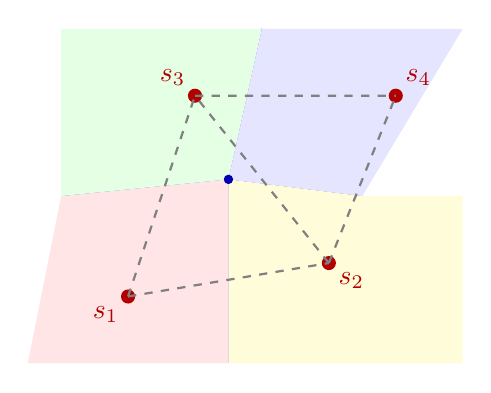
\begin{tikzpicture}[scale=0.85]
  \coordinate (s1) at (0,0);
  \coordinate (s2) at (3,0.5);
  \coordinate (s3) at (1,3);
  \coordinate (s4) at (4,3);
  \draw[blue!60,thick] (-1,1.5)--(1.5,1.75)--(3.5,1.5);
  \draw[blue!60,thick] (1.5,1.75)--(2,4);
  \draw[blue!60,thick] (1.5,1.75)--(1.5,-1);
  \fill[red!10] (-1.5,-1)--(-1,1.5)--(1.5,1.75)--(1.5,-1)--cycle;
  \fill[green!10] (1.5,1.75)--(-1,1.5)--(-1,4)--(2,4)--cycle;
  \fill[blue!10] (1.5,1.75)--(2,4)--(5,4)--(3.5,1.5)--cycle;
  \fill[yellow!15] (1.5,1.75)--(3.5,1.5)--(5,1.5)--(5,-1)--(1.5,-1)--cycle;
  \fill[red!70!black] (s1) circle (3pt) node[below left] {$s_1$};
  \fill[red!70!black] (s2) circle (3pt) node[below right] {$s_2$};
  \fill[red!70!black] (s3) circle (3pt) node[above left] {$s_3$};
  \fill[red!70!black] (s4) circle (3pt) node[above right] {$s_4$};
  \draw[gray,dashed,thick] (s1)--(s2) (s1)--(s3) (s2)--(s3) (s2)--(s4) (s3)--(s4);
  \fill[blue!70!black] (1.5,1.75) circle (2pt);
\end{tikzpicture}
\caption{Voronoi diagram (colored cells) and its Delaunay triangulation dual (dashed gray edges). Each Voronoi vertex is the circumcenter of a Delaunay triangle.}
\label{fig:voronoi_duality}
\end{figure}


\subsection{Pseudocode}

\begin{algorithm}[htbp]
\caption{Voronoi Diagram via Delaunay Dual}
\label{alg:voronoi}
\begin{algorithmic}[1]
\Function{ComputeVoronoi}{sites, bounding\_box}
  \State $DT \gets \text{DelaunayTriangulation}(sites)$
  \State $Circumcenters \gets \{\}$
  \For{$T$ in $DT.triangles$}
    \State $Circumcenters[T] \gets \text{CalculateCircumcenter}(T.v1, T.v2, T.v3)$
  \EndFor
  \State $VoronoiCells \gets [\,]$
  \For{$site$ in $sites$}
    \State $Star \gets \text{FindTrianglesSharingVertex}(site, DT)$
    \State $SortedStar \gets \text{SortAround}(site, Star)$
    \State $CellBoundary \gets [Circumcenters[T] \mid T \in SortedStar]$
    \State $ClippedCell \gets \text{ClipPolygon}(CellBoundary, bounding\_box)$
    \State $VoronoiCells.\text{append}(ClippedCell)$
  \EndFor
  \State \Return $VoronoiCells$
\EndFunction
\end{algorithmic}
\end{algorithm}

\subsection{Parameters}

\begin{itemize}
\item \textbf{Bounding Box}: Essential for ``capping'' the infinite cells belonging to sites on the convex hull.
\item \textbf{Precision}: Circumcenter calculations can be sensitive to nearly collinear sites; robust geometric predicates are recommended.
\end{itemize}

\subsection{Complexity}

\begin{itemize}
\item \textbf{Time Complexity}: $O(n \log n)$\index{time complexity!$O(n \log n)$}, which is the complexity of building the Delaunay triangulation. The extraction of the Voronoi diagram from the triangulation is $O(n)$.
\item \textbf{Space Complexity}: $O(n)$ to store both the triangulation and the resulting Voronoi cells.
\end{itemize}

\subsection{Usages}

\begin{itemize}
\item \textbf{Facility Location}: Determining the optimal placement of a new service center (e.g., a hospital or cell tower).
\item \textbf{Robotics}: Path planning (staying as far away from obstacles as possible by following Voronoi edges).
\item \textbf{Biology/Ecology}: Modeling territory of animals or growth patterns of cells.
\item \textbf{Data Science}: K-nearest neighbors search and clustering.
\end{itemize}

\begin{example}[Voronoi of Two Sites]\label{ex:voronoi_two_sites}
Consider two sites $s_1 = (0, 0)$ and $s_2 = (4, 0)$. The Voronoi diagram consists of two half-planes divided by the perpendicular bisector $x = 2$. Every point with $x < 2$ is closer to $s_1$; every point with $x > 2$ is closer to $s_2$. There is one Voronoi edge (the line $x=2$) and no finite Voronoi vertices.
\end{example}

\subsection{Testing and Edge Cases}

\begin{itemize}
\item \textbf{Sites on Convex Hull}: These cells are naturally open/infinite and require clipping.
\item \textbf{Co-circular Sites}: Four or more points on a circle results in a single Voronoi vertex shared by more than three cells.
\item \textbf{Collinear Sites}: Result in parallel perpendicular bisectors; the Delaunay triangulation may be degenerate.
\item \textbf{Duplicate Sites}: Should be merged or handled to avoid zero-area triangles.
\end{itemize}

\subsection{References}

\begin{itemize}
\item Voronoi, G. (1908). ``Nouvelles applications des param\`{e}tres continus \'{a} la th\'{e}orie des formes quadratiques''. Journal f\"{u}r die reine und angewandte Mathematik.
\item Fortune, S. (1987). ``A sweepline algorithm for Voronoi diagrams''. Algorithmica.
\item Aurenhammer, F. (1991). ``Voronoi Diagrams: A Survey of a Fundamental Geometric Data Structure''. ACM Computing Surveys.
\item Wikipedia: Voronoi diagram.
\end{itemize}


\section{Kinetic Voronoi Diagrams}
\label{sec:kinetic_voronoi}

A kinetic Voronoi diagram\index{kinetic Voronoi diagram} is a data structure that maintains the Voronoi diagram of a set of moving points (sites). Unlike a static Voronoi diagram, where points are fixed, in a kinetic setting, the points move according to known trajectories (e.g., linear or algebraic functions of time). The goal is to update the topological structure of the diagram only at discrete time instances where the Voronoi property is violated.

\subsection{Definitions}

\begin{definition}[Kinetic Data Structure]\label{def:kds}
A \emph{kinetic data structure} (KDS)\index{kinetic data structure} is a framework for maintaining a combinatorial property of a set of moving objects. It consists of certificates that guarantee the current structure is valid, and an event-driven update mechanism.
\end{definition}

\begin{definition}[Certificate]\label{def:certificate}
A \emph{certificate} is a boolean predicate whose truth value guarantees the current topological structure of the kinetic data structure is valid.
\end{definition}

\subsection{Theory}

The maintenance of a kinetic Voronoi diagram is performed through its dual, the \textbf{Kinetic Delaunay Triangulation}.
\begin{enumerate}
\item \textbf{Certificates}: For every edge $(A, B)$ shared by triangles $ABC$ and $ABD$ in the Delaunay triangulation, a certificate is defined based on the \textbf{In-Circle} test: $\operatorname{InCircle}(A(t), B(t), C(t), D(t)) \ge 0$.
\item \textbf{Event Prediction}: The roots of the certificate function (which is typically a polynomial in $t$) are calculated to find the next time $t_{event}$ when the certificate will fail.
\item \textbf{Event Queue}: All predicted event times are stored in a priority queue.
\item \textbf{Topological Update}: When the current time reaches $t_{event}$, an \textbf{Edge Flip} is performed on the corresponding edge, and new certificates are generated for the affected triangles.
\end{enumerate}

This approach is extremely efficient because the number of topological changes is usually much smaller than the number of time steps required for a naive sampling approach.

\subsection{Pseudocode}

\begin{algorithm}[htbp]
\caption{Kinetic Voronoi Maintenance}
\label{alg:kinetic_voronoi}
\begin{algorithmic}[1]
\Function{MaintainKineticVoronoi}{points, trajectories}
  \State $DT \gets \text{DelaunayTriangulation}(points)$
  \State $event\_queue \gets \text{PriorityQueue}()$
  \For{$edge$ in $DT.edges$}
    \State $t\_fail \gets \text{PredictFailureTime}(edge, trajectories)$
    \If{$t\_fail > current\_time$}
      \State $event\_queue.\text{push}(\text{Event}(t\_fail, edge))$
    \EndIf
  \EndFor
  \While{$current\_time < end\_time$}
    \State $event \gets event\_queue.\text{pop}()$
    \State $current\_time \gets event.time$
    \State $edge \gets event.edge$
    \State $new\_edge \gets \text{Flip}(edge, DT)$
    \For{$neighbor$ in $\text{GetAffectedEdges}(new\_edge)$}
      \State $\text{UpdateEvent}(neighbor, event\_queue, trajectories)$
    \EndFor
  \EndWhile
\EndFunction
\end{algorithmic}
\end{algorithm}

\subsection{Parameters}

\begin{itemize}
\item \textbf{Trajectory Model}: Linear ($P(t) = P_0 + vt$) is common, but high-order algebraic paths can be handled using polynomial root solvers.
\item \textbf{Root Finding}: Efficient and robust numerical solvers are needed to find the \emph{first} real root $t > t_{now}$ of the InCircle polynomial.
\end{itemize}

\subsection{Complexity}

\begin{itemize}
\item \textbf{Event Count}: In the worst case, $O(n^2)$\index{time complexity!$O(n^2)$} topological changes for linear trajectories. In practice, it is often close to $O(n)$.
\item \textbf{Processing Time}: $O(\log n)$ per event to update the priority queue and perform the flip.
\end{itemize}

\subsection{Usages}

\begin{itemize}
\item \textbf{Robotics}: Real-time path planning among moving obstacles.
\item \textbf{Crowd Simulation}: Modeling the personal space of individuals in a moving crowd.
\item \textbf{Air Traffic Control}: Tracking the ``empty'' space between moving aircraft.
\item \textbf{Bioinformatics}: Simulating the movement of atoms in a protein or cells in a tissue.
\item \textbf{Astronomy}: Tracking the evolution of cosmic structures over time.
\end{itemize}

\subsection{Testing and Edge Cases}

\begin{itemize}
\item \textbf{Zero Velocity}: Verify that the kinetic structure remains static and produces the same result as the static algorithm.
\item \textbf{Collisions}: Handle cases where two points occupy the same position (distance 0).
\item \textbf{Degenerate Co-circularity}: Multiple events occurring at the exact same time (e.g., points on a square lattice moving synchronously).
\item \textbf{Infinite Time}: Verify that the algorithm handles events predicted far in the future or that never occur.
\item \textbf{Boundary points}: Handle points moving out of the region of interest.
\end{itemize}

\subsection{References}

\begin{itemize}
\item Basch, J., Guibas, L. J., \& Hershberger, J. (1999). ``Data structures for mobile data''. Journal of Algorithms.
\item Guibas, L. J. (1998). ``Kinetic data structures: A new recipe for dynamic geometric algorithms''. ACM SIGART Bulletin.
\item Albers, G., Guibas, L. J., Mitchell, J. S., \& Roos, T. (1998). ``Voronoi diagrams of moving points''. International Journal of Computational Geometry \& Applications.
\item Wikipedia: Kinetic data structure.
\end{itemize}
